\section{Data Technical Debt}
I sistemi AI sono attualmente considerati data-centric, il quale a differenza dei tradizionali sistemi software, i risultati e la qualità del loro modello dipendono principalmente dai dati piuttosto che il codice \cite{KhomhSE4ML}.
E' necessario quindi comprendere le possibili minacce che possono andare a inficiare la qualità dei dati.
In questo contesto,in uno studio condotto da Foidl et al \cite{FoidlDataSmells}, è stata scoperta la presenza di 36 smells che sono presenti nello stato dell'arte. 
I data smells sono poi categorizzati in base alla loro semantica, sintassi e livello di comprensibilità come segue (Figura \ref{fig:data_smells}):
\begin{itemize}
    \item Believability Smells: relativo alla semantica applicata sui valori dei dati. Questa tipologia di smell indica una bassa "credibilità", dovuta spesso all'utilizzo di valori implausibili. Un esempio di istanza di questa categoria di smell è il \textit{dummy value}, dove viene utilizzato un valore ambiguo per la rappresentazione di un valore mancante. Si consideri ad esempio l'utilizzo del valore "999" per la rappresentazione di un dato mancante. Questo valore può essere facilmente interpretato male a seconda del contesto in cui viene applicato, come nel caso in cui il valore è associato al numero telefonico, esso potrebbe essere interpretato come un numero di emergenza.
    \item Understandability Smells: relativo alla sintassi inappropriata o ambigua dei dati. Questa tipologia di smell può creare problemi di lettura e di elaborazione al software. Un tipo esempio è \textit{l'encoding smell}, in cui un inappropriato tipo assegnato al valore dei dati impedisce di poter fare operazioni su di esso.
    \item Consistency Smells: relativo all'uso inconsistente del formato, del tipo e della rappresentazione dei dati. Un tipico esempio è l'\textit{abbreviation inconsistency} in cui la rappresentazione del valore tramite abbreviazioni o acronimi non è utilizzato in modo consistente in tutti i valori dei dati.
\end{itemize}
\begin{figure}[h]
    \centering
    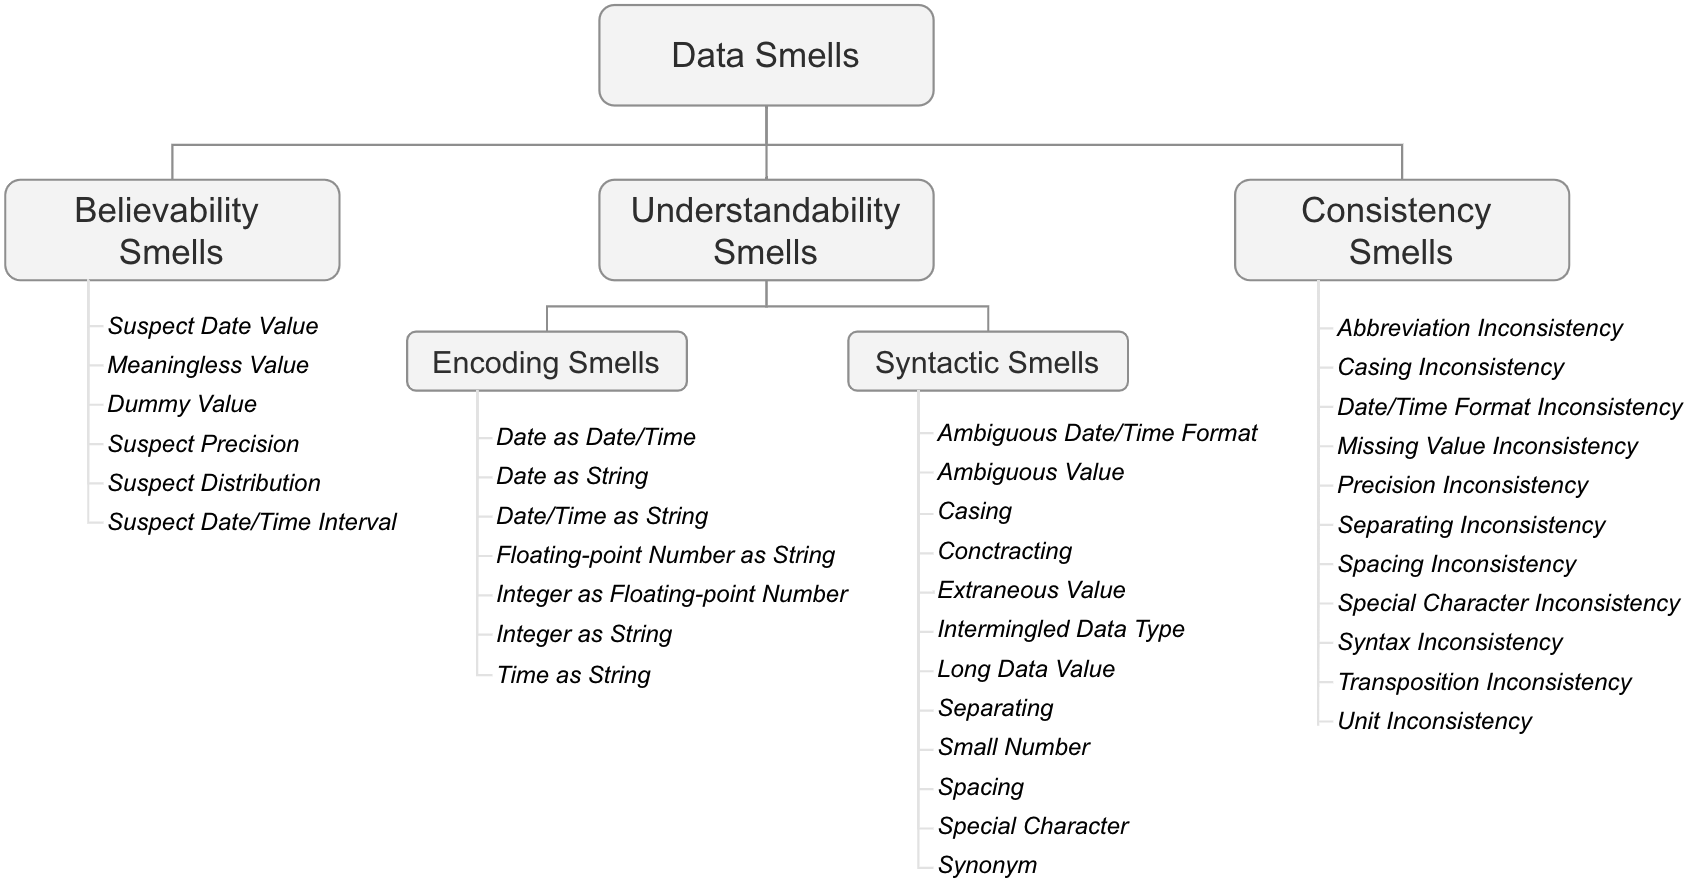
\includegraphics[width=\textwidth]{Figure/StateofArt/data_smell_categories.png}
    \caption{Categorie di Data smells}
    \label{fig:data_smells}
\end{figure}

Inoltre, la rappresentazione inappropriata dei dati non è l'unica minaccia alla qualità del software AI. Secondo uno studio condotto da Sharma et al. \cite{SharmaDBSmells}, anche la violazione di best practice relative alla progettazione di uno schema dei dati può essere causa di introduzione di technical debt nei sistemi. 
Il debito accumulato da una cattiva progettazione dello schema dei dati, come accordato da Al-Barak et al. \cite{Al-BarakDBDebt}, può impattare negativamente non solo sulla qualità, la manutenibilità e l'evoluzione dello schema, ma può inficiare negativamente l'intero sistema.
